\section{Prerequisites}

\subsection{Notation}
\noindent\textbf{Vectors and Matrices.} In this paper, lowercase letters are used to denote vectors, whereas capital letters are used for matrices. 

\noindent\textbf{Transpose of Vectors and Matrices.} The transpose of a vector or a matrix is an operation whereby the rows and columns of the vector or matrix are inverted, and this is denoted using the notation $v^\T$ or $M^\T$. For example:
\[
    \begin{bmatrix}
        a & b \\
        c & d
    \end{bmatrix}^\T
    =
    \begin{bmatrix}
        a & c \\
        b & d
    \end{bmatrix}
\]

\subsection{Homogenous Coordinates} \label{sec:homogenous}

While Euclidean space describes 2D and 3D space well, they are not sufficient in describing perspective projections, as it is unable to fully the capture the relationships inherent in projective projections and affine transformations, both of which are core concepts in this paper. 

Homogenous coordinates forms the basis of projective geometry, because it unifies the treatment of common graphical transformations such as rotation and translations \footcite[][1]{bloomenthalHomogeneousCoordinates1994}. 

Given a point in with coordinates $(a_1, a_2, \cdots, a_n) \in \Real^n$ 



Given the vector $[\,u, v\,]^\T \in \Real^2$, we can express it in terms of homogenous coordinates: 
\begin{equation}
    \begin{bmatrix}
        u \\ v \\ 1
    \end{bmatrix}
    \sim
    \begin{bmatrix}
        u\widetilde{w} \\ v\widetilde{w} \\ \widetilde{w}
    \end{bmatrix}
    \equiv
    \begin{bmatrix}
        \widetilde{u} \\ \widetilde{v} \\ \widetilde{w}
    \end{bmatrix}
\end{equation}

\begin{figure}[H]
    \centering
    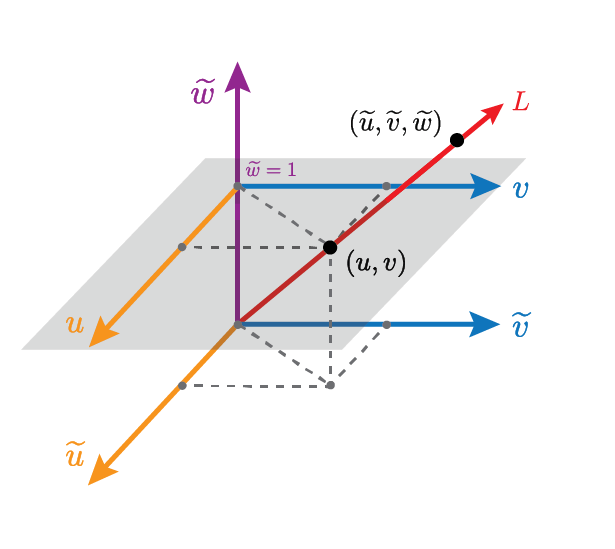
\includegraphics[width=0.6\textwidth]{diagrams/homogenous}
    \caption{Homogenous coordinate system.}
\end{figure}

In other words, with homogenous coordinates, we interpret our \emph{Euclidean} space as an \emph{affine} space
